\documentclass[11pt,a4paper]{article}
\usepackage[a4paper,margin=2.6cm]{geometry}
\usepackage{iftex}
\ifPDFTeX
  \usepackage[T2A]{fontenc}
  \usepackage[utf8]{inputenc}
  \usepackage[russian]{babel}
\else
  \usepackage{fontspec}
  \usepackage{polyglossia}
  \setdefaultlanguage{russian}
  \setotherlanguage{english}
  \defaultfontfeatures{Ligatures=TeX}
  % Font chain: local Times New Roman -> Liberation (Overleaf) -> CMU.
  \IfFontExistsTF{Times New Roman}{%
    \setmainfont{Times New Roman}%
    \setsansfont{Arial}%
    \setmonofont{Courier New}%
    \newfontfamily\cyrillicfont{Times New Roman}%
    \newfontfamily\cyrillicfontsf{Arial}%
    \newfontfamily\cyrillicfonttt{Courier New}%
  }{%
    \IfFontExistsTF{Liberation Serif}{%
      \setmainfont{Liberation Serif}%
      \setsansfont{Liberation Sans}%
      \setmonofont{Liberation Mono}%
      \newfontfamily\cyrillicfont{Liberation Serif}%
      \newfontfamily\cyrillicfontsf{Liberation Sans}%
      \newfontfamily\cyrillicfonttt{Liberation Mono}%
    }{%
      \setmainfont{CMU Serif}%
      \setsansfont{CMU Sans Serif}%
      \setmonofont{CMU Typewriter Text}%
      \newfontfamily\cyrillicfont{CMU Serif}%
      \newfontfamily\cyrillicfontsf{CMU Sans Serif}%
      \newfontfamily\cyrillicfonttt{CMU Typewriter Text}%
    }%
  }
\fi
\usepackage{microtype}
\usepackage{mathtools,amssymb}
\usepackage{graphicx}
\usepackage{booktabs}
\usepackage{float}
\usepackage{caption}
\captionsetup{font=small,labelfont=bf}
\usepackage{enumitem}
\setlist{nosep,leftmargin=1.5em}
\usepackage{csquotes}
\usepackage[backend=biber,style=gost-numeric,sorting=none]{biblatex}
\addbibresource{references_v2.bib}
\usepackage[unicode,hidelinks]{hyperref}
\setlength{\emergencystretch}{2em}

\title{{\normalsize\normalfont\hspace*{-\leftskip}\parbox{\linewidth}{\raggedright УДК~551.513}}\\[1.5em]
Сопряжённость иерархических уровней атмосферной циркуляции\\
как региональный инвариант}
\author{Сотириади Н.}
\date{2026}

\begin{document}
\maketitle

\begin{abstract}
Иерархическая организация геосистем --- одно из оснований отечественной теоретической географии: уровни организации выделяются по спектральным и фрактальным свойствам полей, а программа поиска инвариантов динамики геосистем требует устойчивых числовых характеристик устройства территории. Открытым оставался вопрос об измерении \emph{взаимодействия} выделенных уровней. В работе по полю относительного вихря на поверхности 850~гПа (реанализ ERA5; 12 основных областей с тремя периодами 2017--2024~гг. и 27 контрольных областей) построен профиль сопряжённости соседних октавных уровней~$P$ --- мера того, насколько размещение мезомасштабной изменчивости предопределено соседним крупным уровнем, --- и проверен его статус регионального инварианта в операциональном смысле: устойчивость на заранее заданном классе преобразований условий наблюдения (сезон, независимый год, фаза ЭНСО, источник данных, схема разбиения территории) при значимости $p=0{,}001$ на выборках, не участвовавших в построении величины. Профиль содержит воспроизводимую информацию сверх спектра мощности поля (контроль равновеликими по площади областями: $p=0{,}033$), а его география воспроизводится в свободном модельном расчёте, не усваивающем атмосферных наблюдений (ранговая корреляция 0,71 при внутреннем пределе метода 0,93), --- наблюдаемая структура не объясняется только устройством наблюдательной сети. Наибольшая сопряжённость свойственна внетропическим штормовым путям, наименьшая --- влажно-конвективным режимам; бассейны Конго и Амазонии различаются архитектурой иерархии при близких стандартных характеристиках режима. Полученная величина дополняет аппарат районирования характеристикой устройства межуровневых связей; её прикладное содержание для задач прогноза на сегодняшних данных не установлено, границы применимости перечислены явно.

\smallskip
\noindent\textbf{Ключевые слова:} иерархическая организация геосистем, инварианты, масштаб, атмосферная циркуляция, реанализ, районирование, генерализация.
\end{abstract}

\section{Введение}
\label{sec:intro}

\subsection{Инварианты организации территории}

Представление о геосистемах как об иерархически организованных образованиях, в которых процессы разных пространственно-временных уровней связаны, но не сводимы друг к другу, принадлежит к числу основополагающих в отечественной теоретической географии. В работах Ю.\,Г.~Пузаченко эта идея получила операциональное развитие: пространственно-временная иерархия геосистем рассмотрена с позиций теории колебаний \cite{Puzachenko1986}, сформирован аппарат выделения уровней организации по спектральным и фрактальным свойствам географических полей \cite{Puzachenko2004}, а поиск \emph{инвариантов динамики геосистем} --- устойчивых во времени числовых характеристик организации, различающих территории, --- поставлен как самостоятельная исследовательская программа \cite{Puzachenko2010}. Инвариант в этом понимании не есть константа природы; это воспроизводимая мера устройства территории, сохраняющая значение при смене состояния системы и потому пригодная для сравнения и районирования.

Непосредственным развитием линии стала работа А.\,Н.~Кренке с соавторами \cite{Krenke2019}, где иерархические уровни организации регионального мезоклимата выделялись по двумерным спектрам главных компонент климатических полей. Тем самым получен ответ на вопрос, \emph{где} расположены уровни организации. Следующий по логике вопрос --- как измерить \emph{отношение} между уровнями: насколько размещение изменчивости одного уровня предопределено соседним. Величины такого рода до сих пор не строились как самостоятельные характеристики территории и не проверялись на статус инвариантов. Настоящая работа посвящена этому вопросу применительно к атмосферной циркуляции.

\subsection{Чего не измеряют существующие подходы}

Близкие по духу инструменты развивались в трёх традициях, и каждая оставляет искомую величину за пределами рассмотрения. Каскадные и мультифрактальные описания \cite{LovejoySchertzer2013,Lovejoy2011,Kouhen2024} характеризуют распределение интенсивности \emph{вдоль} масштабного континуума, но не пространственную согласованность карт активности \emph{между} конкретными уровнями. Вейвлет-огибающие и их статистики --- коэффициент амплитудной модуляции \cite{Farge1992,Mathis2009} и систематизирующие его скаттеринг-ковариации (статистики рассеивающего вейвлет-преобразования) \cite{Mallat2012,BrunaMallat2013,Cheng2024} --- измеряют факт связи уровней, но применялись как признаки для классификации, а не как климатология устройства территории; одно из недавних приложений подобной техники к различению режимов геофизических полей --- океанологическая работа \cite{Skinner2025}. Наконец, литература о предсказуемости атмосферы \cite{Lorenz1969,Zhang2007,RotunnoSnyder2008,Judt2020,SelzCraig2023} отводит межмасштабному взаимодействию роль канала, по которому неопределённость мелких масштабов заражает синоптический уровень, но \emph{моделирует} силу этой связи, а не измеряет её по данным.

Сама форма оценки --- корреляция огибающих соседних полос одного поля --- при этом не нова. Её ближайший формальный родственник --- корреляция амплитудных огибающих частотных полос, введённая в нейрофизиологии для выявления связи некогерентных компонент сигнала \cite{Bruns2000}; в той же дисциплине изучается и более широкий класс межчастотных связей, включая конструктивно иную, фазо-амплитудную связь \cite{Canolty2006}. Родственная, но конструктивно иная форма --- корреляция крупномасштабного \emph{сигнала} с огибающей мелких масштабов (коэффициент амплитудной модуляции) --- независимо сложилась в физике пристеночной турбулентности \cite{Mathis2009}. Независимое появление родственных форм в разных дисциплинах подчёркивает естественность конструкции, но не отвечает ни на вопрос о её содержании для конкретного географического поля, ни на вопрос о статусе инварианта; прямое сопоставление предложенного дескриптора с этими родственниками выполнено и обсуждается в разд.~\ref{sec:estimator}.

\subsection{Операциональное определение проверяемого утверждения}
\label{sec:definition}

Слово <<инвариант>> в заглавии требует точного определения того, чт\'{о} проверяется. Пусть $P^{(\ell)}_{G;\,\tau}$ --- значение профиля сопряжённости области $G$ на масштабной ступени $\ell$ при условиях наблюдения $\tau=(s,y,e,d,g)$: сезон $s$, год $y$, фаза ЭНСО $e$, источник данных $d$, схема разбиения территории $g$. Проверяемое утверждение --- \emph{условная инвариантность на заранее заявленном классе преобразований} $\mathcal{T}$:
\begin{equation}
P^{(\ell)}_{G;\,\tau}\approx P^{(\ell)}_{G;\,\tau'}
\quad\text{для всех }\tau,\tau'\in\mathcal{T},
\label{eq:invariance}
\end{equation}
при том что межрегиональные различия профилей остаются существенно больше внутрирегиональных (форма утверждения в терминах кластеризации, разд.~\ref{sec:inference}). Класс $\mathcal{T}$ зафиксирован протоколами до вычислений и включает: смену сезона (январь--март~/ июль--сентябрь), смену независимого года, смену фазы ЭНСО, смену источника данных (ERA5~/ MERRA-2~/ свободный модельный расчёт) и смену схемы разбиения территории (градусные~/ равновеликие области).

Столь же явно фиксируются \emph{границы} утверждения. Оно относится: к полю относительного вихря (не к произвольной атмосферной переменной); к уровню 850~гПа (перенос на 500~гПа не подтверждён, разд.~\ref{sec:meaning}); к изученным областям и широтам; преимущественно к разрешённым ступеням 4--5, обе полосы которых не мельче 200~км (эффективное разрешение реанализов, разд.~\ref{sec:data}); к временным окнам 2017--2024~гг. Динамическая автономность величины и её прогностическая полезность в класс проверенных свойств \emph{не входят}: соответствующие гипотезы проверены и не подтвердились (разд.~\ref{sec:meaning}). Далее термин <<региональный инвариант>> употребляется исключительно как сокращение утверждения~\eqref{eq:invariance} с перечисленными границами --- в операциональном смысле традиции \cite{Puzachenko2010}, а не как заявка на универсальный закон.

\subsection{Задачи}

(1)~Построить по полю относительного вихря компактный дескриптор межуровневой организации --- профиль сопряжённости уровней~$P$ --- с полным операциональным описанием процедуры оценивания. (2)~Проверить утверждение~\eqref{eq:invariance} на классе $\mathcal{T}$, с защитой от артефактов геометрии выборки и наблюдательной системы. (3)~Установить, что дескриптор измеряет и чего не измеряет, включая перечень проверенных и отвергнутых интерпретаций.

\section{Материалы и методы}
\label{sec:data}

\subsection{Данные}

Основной материал --- реанализ ERA5 \cite{Hersbach2020,Soci2024}: составляющие ветра на поверхности 850~гПа, сетка $0{,}25^\circ$, шаг 6~ч. Выбор уровня 850~гПа отвечает его представительности для нижнетропосферной циркуляции, непосредственно взаимодействующей с подстилающей поверхностью.

Анализ ведётся в 39 областях размером $20^\circ$ широты $\times\ 40^\circ$ долготы. Двенадцать из них выбраны содержательно \emph{до начала анализа} и покрывают шесть контрастных циркуляционных режимов: тропические океаны, внетропические штормовые пути обоих полушарий, очаги глубокой конвекции над сушей и континентальные области умеренного и субтропического поясов. Остальные 27 заданы формальным правилом, зафиксированным до получения данных: фиксированная решётка ячеек $20^\circ\times40^\circ$ (пять широтных полос от $55^\circ$~с.\,ш. до $45^\circ$~ю.\,ш., долготные грани через $40^\circ$ от $20^\circ$~в.\,д.; 45 ячеек) с исключением ячеек, перекрывающихся с основными областями более чем на 20\,\% площади, --- чтобы состав выборки нельзя было заподозрить в подгонке; решёточные области используются только для проверки географии на независимом составе выборки (2024~г.). Для двенадцати основных областей привлечены три периода: 2017--2019~гг. (области R1--R4, 16 регион-окон, использованных при постановке метода), 2021--2022~гг. (области R5--R12, 32 регион-окна) и 2023--2024~гг. (все 12 областей, 48 регион-окон); каждая область в итоге располагает восемью сезонными окнами. Периоды охватывают Ла-Нинью (2021--2022~гг.), Эль-Ниньо (2023--2024~гг.) и преимущественно нейтральные условия (2017--2019~гг.). Проверки кластеризации строятся на 48 основных регион-окнах; 32 окна 2021--2022~гг., охватывающие восемь из двенадцати областей, служат отложенной выборкой, не участвовавшей в построении дескриптора.

Для проверки воспроизводимости привлечены два внешних источника. Первый --- реанализ MERRA-2 \cite{Gelaro2017}, построенный на другой модели общей циркуляции и другой системе усвоения, но использующий в основном ту же наблюдательную базу: эта проверка квазинезависима --- она исключает артефакты конкретной системы усвоения, но не наблюдательной сети как таковой. Второй --- эксперимент \texttt{highresSST-present} проекта HighResMIP \cite{Haarsma2016} по модели ECMWF-IFS-HR \cite{Roberts2018}: расчёт с заданной наблюдаемой температурой поверхности океана, \emph{не усваивающий никаких атмосферных наблюдений}. Использованы сезонные окна января--марта и июля--сентября 2014~г. --- последнего года эксперимента (протокол охватывает 1950--2014~гг.), поэтому сопоставление с окнами ERA5 2017--2024~гг. по построению климатологическое: сравниваются устойчивые географии, а не совпадающие годы.

Ограничение материала оговаривается заранее, и оценки его строгости расходятся: правило 4--7 шагов сетки \cite{Skamarock2004} даёт для ERA5 эффективное разрешение около 125--220~км, тогда как прямая спектральная оценка \cite{Bolgiani2022} --- 500--600~км в средних широтах и порядка 1000~км в тропиках. Изменчивость мелких ступеней лестницы, таким образом, в значительной мере формируется численной диссипацией и параметризациями. Поэтому, во-первых, все основные выводы дублируются контролем, ограниченным ступенями, обе полосы которых не мельче 200~км (умеренный порог по правилу 4--7 шагов; формальное определение разрешённых ступеней --- разд.~\ref{sec:estimator}), и сопоставление с внешними источниками ведётся только по ним; во-вторых, решающие проверки природы сигнала --- суррогатная поправка и воспроизведение географии в другом реанализе и в свободном расчёте --- от выбора порога не зависят: в них сравниваются поля, прошедшие один и тот же вычислительный тракт.

\subsection{Процедура оценивания и измеряемая величина}
\label{sec:estimator}

Дескриптор строится в семь шагов; все параметры вычислительной схемы (табл.~\ref{tab:params}) зафиксированы протоколом до вычислений и едины для всех областей, источников данных и проверок.

\begin{enumerate}
\item \emph{Поле.} По составляющим ветра вычисляется относительный вихрь $\omega=\partial v/\partial x-\partial u/\partial y$ с широтно-зависимой километровой метрикой сферы. Вихрь предпочтительнее составляющих ветра тем, что подчёркивает вращательную структуру течения и подавляет крупномасштабный адвективный фон.
\item \emph{Масштабные уровни.} Для лестницы масштабов $\ell\in\{50,100,200,400,800,1600\}$~км строятся изотропные гауссовы сглаживания $\overline{\omega}_{\ell}$ с $\sigma=\ell/\sqrt{12}$ (дисперсионный эквивалент прямоугольного окна ширины $\ell$); ширина ядра в узлах сетки адаптируется к широтной метрике построчно. Уровень~$i$ ($i=1,\dots,5$) --- разность соседних сглаживаний (октава):
\begin{equation}
D_i(x,y,t)=\overline{\omega}_{\ell_i}-\overline{\omega}_{\ell_{i+1}}.
\end{equation}
Нулевой уровень --- остаток мельче первого масштаба, $D_0=\omega-\overline{\omega}_{50}$; всего, таким образом, шесть уровней $D_0,\dots,D_5$. Такое разложение идейно соответствует выделению уровней организации по спектру \cite{Krenke2019}, но переносит анализ в физическое пространство.
\item \emph{Карты активности.} Огибающая уровня --- модуль $D_i$, сглаженный на крупном краю его октавы (для нулевого уровня --- при $\sigma=\ell_1/\sqrt{12}$):
\begin{equation}
E_i(x,y,t)=\overline{\lvert D_i\rvert}_{\ell_{i+1}},
\end{equation}
она показывает, \emph{где} в срок $t$ сосредоточена изменчивость уровня; шести уровням отвечают огибающие $E_0,\dots,E_5$. Использование огибающих как индикаторов локальной активности масштаба восходит к вейвлет-анализу турбулентности \cite{Farge1992}.
\item \emph{Корреляция соседних уровней.} Для каждого 6-часового срока $t$ по узлам внутренней маски области (краевая полоса шириной $\min(2\ell_{\max};\,0{,}25$ размера области$)$ исключена) вычисляется пространственная ранговая корреляция логарифмов огибающих:
\begin{equation}
\rho_i(t)=\operatorname{corr}_{\mathrm{rank}}\!\left[\ln\!\big(E_{i-1}+\varepsilon\big),\ \ln\!\big(E_{i}+\varepsilon\big)\right],
\qquad \varepsilon=10^{-12}\ \text{с}^{-1}.
\label{eq:rho}
\end{equation}
Пять ступеней профиля $i=1,\dots,5$ отвечают пяти парам соседних огибающих $(E_{i-1},E_i)$, то есть парам полос: 1~--- (мельче~50; 50--100~км), 2~--- (50--100; 100--200~км), 3~--- (100--200; 200--400~км), 4~--- (200--400; 400--800~км), 5~--- (400--800; 800--1600~км). \emph{Разрешёнными} далее называются ступени 4--5 --- единственные, у которых обе полосы пары не мельче 200~км.
\item \emph{Агрегирование во времени.} Профиль области в окне --- медиана $\rho_i(t)$ по всем срокам сезонного окна ($\approx$360 сроков); $P=(\rho_1,\dots,\rho_5)$.
\item \emph{Суррогатный фон.} Перекрытие соседних гауссовых октав само по себе даёт ненулевую сопряжённость даже для случайного поля с тем же спектром. Поэтому для каждого регион-окна генерируется ансамбль фазовых суррогатов \emph{исходного поля ветра}: на каждом сроке спектры $u$ и $v$ умножаются на общее случайное фазовое поле (амплитудный спектр каждой составляющей и среднее по области сохраняются точно; общая фаза сохраняет взаимную когерентность $u$ и $v$), после чего вся последовательность операций (шаги~1--5) повторяется на суррогате. Порядок операций строго <<суррогат~$\to$~фильтрация>>. Рандомизация выполняется на прямоугольнике области без оконной функции; краевые эффекты преобразования одинаковы для реального и суррогатного полей, проходящих один и тот же тракт, и дополнительно подавляются внутренней маской (шаг~4). Отметим, что в силу линейности оператора вихря умножение спектров $u$ и $v$ на общий фазовый множитель умножает на него и спектр $\omega$: процедура тождественна фазовой рандомизации самого поля вихря с точным сохранением его пространственного спектра.
\item \emph{Суррогатная поправка.} Основная форма дескриптора --- превышение над медианой суррогатного ансамбля, $P-P_{\mathrm{surr}}$ (далее --- профиль с суррогатной поправкой): оно свободно от вклада перекрытия фильтров и отражает собственно негауссову организацию поля. Исходный профиль (без поправки) приводится параллельно во всех проверках.
\end{enumerate}

\begin{table}[H]
\centering
\caption{Параметры процедуры оценивания (зафиксированы до начала вычислений).}
\label{tab:params}
\small
\begin{tabular}{@{}p{0.40\linewidth}p{0.54\linewidth}@{}}
\toprule
Параметр & Значение\\
\midrule
Поле & относительный вихрь, 850~гПа, метрика сферы\\
Сетка и шаг по времени & $0{,}25^\circ$; 6~ч; окно $\approx$360 сроков (91 сут $\times$ 4)\\
Лестница масштабов $\ell$ & 50, 100, 200, 400, 800, 1600~км (октавы)\\
Фильтр уровня & изотропный гауссов, $\sigma=\ell/\sqrt{12}$, построчная адаптация к широтной метрике\\
Огибающая $E_i$ & $\lvert D_i\rvert$, сглаженный при $\sigma=\ell_{i+1}/\sqrt{12}$\\
Регуляризация логарифма & $\ln(E+\varepsilon)$, $\varepsilon=10^{-12}$~с$^{-1}$\\
Область корреляции & узлы внутренней маски области; краевая полоса $\min(2\ell_{\max};\,0{,}25$ размера области$)$ исключена\\
Форма корреляции & ранговая (Спирмена); линейная форма даёт $\rho=0{,}99$ с ранговой (см. текст)\\
Агрегирование & медиана по срокам окна\\
Суррогаты & фазовая рандомизация поля ветра, общее фазовое поле для $u$ и $v$; 199 реализаций на регион-окно; поправка по медиане ансамбля\\
\bottomrule
\end{tabular}
\end{table}

Три пояснения к описанной процедуре. Во-первых, корреляционная форма на логарифмах огибающих делает дескриптор нечувствительным к региональным различиям общей интенсивности циркуляции; как показано в разд.~\ref{sec:meaning}, именно нечувствительность к амплитуде отличает работоспособную конструкцию от неработоспособной. Во-вторых, выбор \emph{ранговой} корреляции --- техническая деталь реализации, повышающая устойчивость оценки, а не содержательная часть нового объекта: замена ранговой корреляции линейной корреляцией логарифмов огибающих воспроизводит географию дескриптора практически тождественно ($\rho=0{,}99$ между двумя вариантами оценки), поэтому никакая часть новизны не приписывается <<ранговости>> конструкции. В-третьих, суррогатная поправка отвечает на критику родственного коэффициента амплитудной модуляции: в \cite{CuiJacobi2025} показано, что тот отражает главным образом линейное взаимодействие со средним потоком, а не собственно межмасштабную связь. Здесь искомая часть сигнала выделяется контролем: поправка сравнивает наблюдаемую сопряжённость с полем той же спектральной структуры и удаляет весь вклад второго порядка по построению. Прямое сопоставление с самим коэффициентом амплитудной модуляции выполнено: на общем материале он статистически отличен от $P$ (ранговая корреляция карт $+0{,}14$) и не воспроизводит устойчивой региональной географии --- то есть предложенный дескриптор не является переименованием известной статистики.

\emph{Выполненные вариации процедуры оценивания.} Устойчивость результатов проверена к следующим изменениям вычислительной схемы: ранговая~/ линейная корреляция ($\rho=0{,}99$); профиль с суррогатной поправкой~/ исходный профиль (обе формы во всех проверках); ограничение разрешёнными ступенями 4--5 ($p=0{,}002$, разд.~\ref{sec:artifacts}); вариация протяжённости равновеликих областей $\pm10\,\%$ (согласие профилей по каждому региону $\rho\ge0{,}93$); замена фиксированной километровой лестницы на масштабированную локальным радиусом деформации ($p=0{,}001$). Чувствительность к семейству фильтров, ширине сглаживания огибающей и отношению соседних масштабов отдельно не варьировалась: эти параметры зафиксированы до начала вычислений, что исключает их подгонку под результат (обсуждение --- разд.~\ref{sec:limitations}).

\subsection{Схема статистического вывода}
\label{sec:inference}

Исследование построено по фальсификационной схеме: критерии и единственная статистика каждой проверки фиксировались \emph{до} обращения к соответствующим данным (полные протоколы и журнал отступлений открыты в репозитории, см. <<Данные и код>>), а ключевые утверждения подтверждались на выборках, не участвовавших в их получении. Ниже указаны единицы вывода и нуль-модели --- защита от псевдорепликации.

\emph{Единица вывода} --- регион-окно: медианное агрегирование по $\approx$360 срокам (шаг~5 схемы) сводит каждое сезонное окно области к одному пятимерному вектору, так что внутриоконная временная зависимость сроков устраняется агрегированием и в статистику не входит. Число регион-окон (48 основных, 32 отложенных) используется как операционная единица анализа, но является верхней оценкой эффективного числа независимых единиц (см. ограничения ниже); числом сроков оно не является заведомо.

\emph{Перестановочный тест кластеризации.} Дескрипторы стандартизуются покомпонентно (приведение к нулевому среднему и единичной дисперсии по выборке); статистика --- разность медианных попарных евклидовых расстояний <<между регионами>> и <<внутри регионов>>, $\Delta=\mathrm{med}_{\mathrm{between}}-\mathrm{med}_{\mathrm{within}}$; $\Delta$ измеряется в единицах стандартизованного пространства дескрипторов и приводится всюду рядом с $p$ как размер эффекта. Нуль-модель --- 999 случайных переназначений региональных меток целым регион-окнам; $p=(1+\#\{\Delta^\ast\ge\Delta\})/1000$, поэтому минимально достижимое значение равно $p=0{,}001$. Региональные метки заданы составом выборки до анализа. Межгодовая согласованность окон одного региона --- не мешающий фактор, а само проверяемое свойство~\eqref{eq:invariance}; перестановке подвергаются целые окна, а не сроки.

\emph{Несводимость к более простым характеристикам} проверяется на регрессионных остатках (схема с исключением по одному): из дескриптора удаляется часть, линейно предсказуемая по контрольному набору признаков (спектральные признаки; полуфрактальные характеристики уровней --- прямые аналоги признаков выделения уровней в \cite{Krenke2019}; скаттеринг-статистики второго порядка \cite{Cheng2024}; геометрия области), после чего тест кластеризации повторяется на остатках.

\emph{Контроль геометрии построением выборки.} Помимо регрессионного контроля выполнен контроль конструкцией: те же двенадцать регионов заново нарезаны равновеликими областями $2000\times2800$~км (те же центры, индексные маски на исходной сетке), и вся последовательность операций --- включая повторное построение фазовых суррогатов для каждого окна --- повторена на 48 основных и 32 отложенных регион-окнах. В отличие от регрессии ковариат, такой контроль устраняет широтную зависимость километровой геометрии из самого построения выборки и потому не может поглотить вместе с геометрией физический сигнал, коррелированный с широтой. Равновеликие области близки по площади к среднеширотным градусным и меньше экваториальных ($5{,}6$ против $9{,}9$~млн~км$^2$): цель контроля --- равенство площадей между регионами, а не сохранение исходной площади каждой области.

\emph{Признаваемые ограничения схемы.} Перестановка региональных меток не моделирует явно пространственную корреляцию соседних областей, а окна одного региона разделяют режим и географию, поэтому число регион-окон --- верхняя оценка числа независимых единиц (консервативная нижняя --- число областей); усилением схемы были бы исключение целых регионов и блочный бутстреп по синоптическим отрезкам. Поправка на множественность проверок не вводилась: каждая строка табл.~\ref{tab:tests} отвечает отдельной, заранее заявленной гипотезе со своей, также заранее заявленной статистикой; значения на границе значимости ($p=0{,}026$--$0{,}033$) следует читать с обеими оговорками. Наконец, на верхней ступени внутренняя часть области вмещает лишь несколько корреляционных радиусов, что ограничивает точность отдельных значений $\rho_5$; значимость при этом оценивается перестановками целых окон, а не узлов сетки. Ключевые утверждения работы опираются на результаты с $p=0{,}001$ и большими размерами эффекта ($\Delta>1$), устойчивые к разумным поправкам эффективного объёма выборки.

\section{Результаты}
\label{sec:results}

\subsection{Карта сопряжённости уровней}
\label{sec:map}

Профиль сопряжённости монотонно убывает от мелких уровней к крупным во всех областях, но скорость убывания и уровень, на котором происходит основная потеря связи, различаются регионально и устойчиво (рис.~\ref{fig:profiles}).

\begin{figure}[H]
\centering
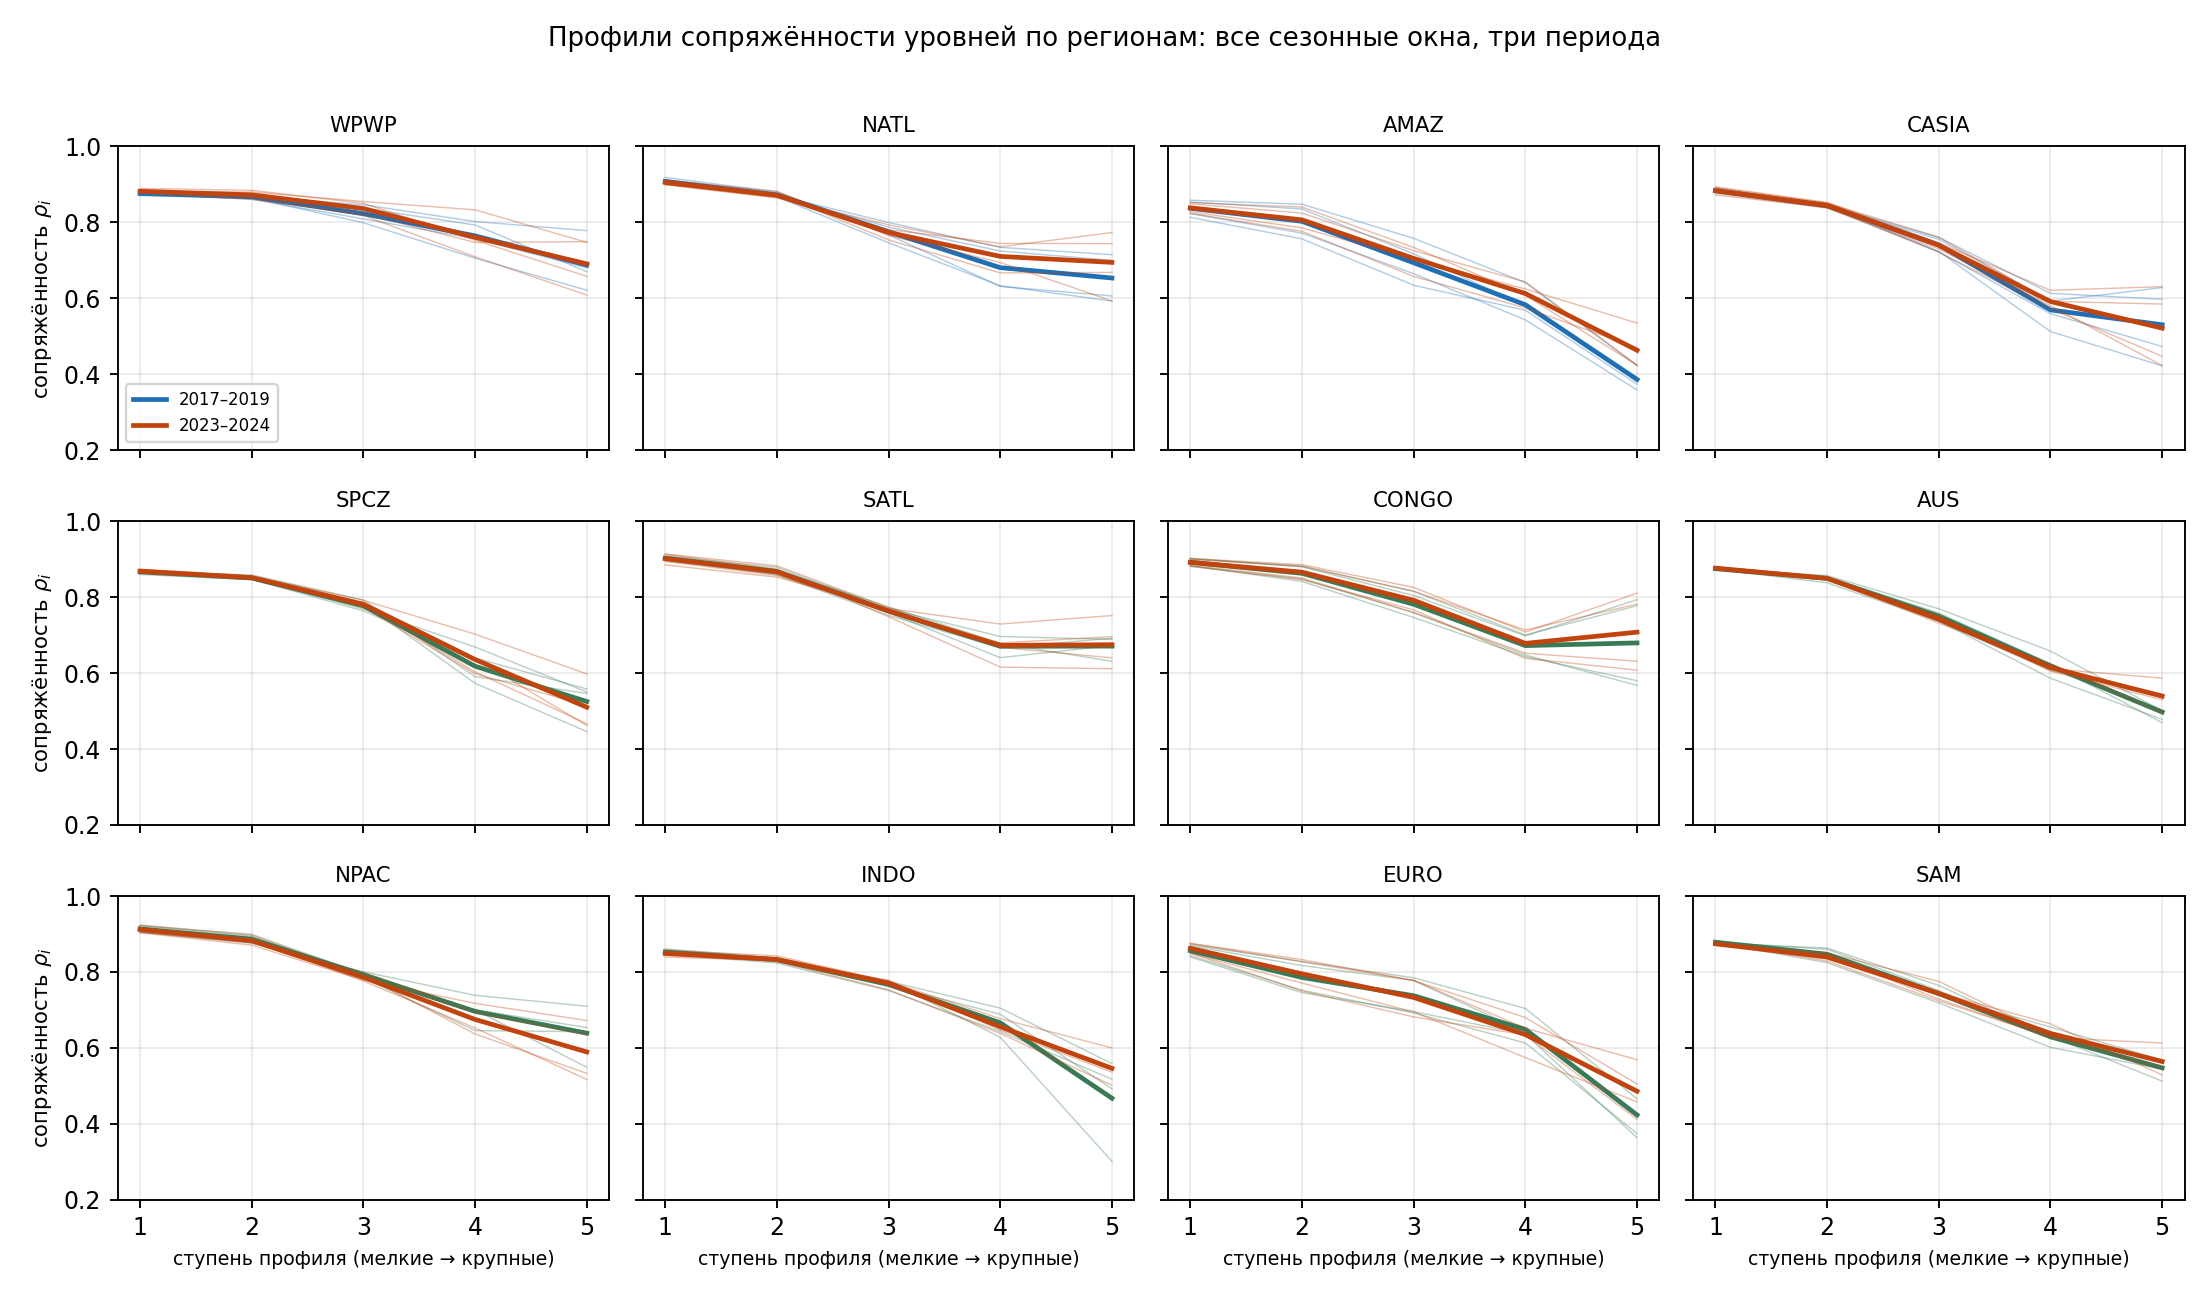
\includegraphics[width=\linewidth]{figures/figP_profiles.png}
\caption{Профили сопряжённости уровней $P$: тонкие линии --- отдельные сезонные окна, жирные --- средние по периодам 2017--2019, 2021--2022 и 2023--2024~гг. Ступени 1--5 отвечают парам соседних уровней: от (мельче~50; 50--100~км) до (400--800; 800--1600~км).}
\label{fig:profiles}
\end{figure}

Среднее значение профиля по разрешённым ступеням 4--5 меняется по областям от 0,51 (Амазония) до 0,73 (рис.~\ref{fig:pmap}); значения отдельных ступеней выходят за этот диапазон. География читается содержательно. Наибольшая сопряжённость свойственна внетропическим штормовым путям: фронтальная структура согласованно проявляется на всех уровнях, и по крупномасштабному полю можно указать, где расположится мезомасштаб. Наименьшая --- влажно-конвективным океаническим режимам, где мезомасштабная организация порождается процессами, слабо определяемыми крупномасштабным полем. Континентальные области умеренного пояса занимают промежуточное положение. Это прочтение --- содержательная гипотеза (разд.~\ref{sec:geo}), а не установленный в настоящей работе факт.

\begin{figure}[H]
\centering
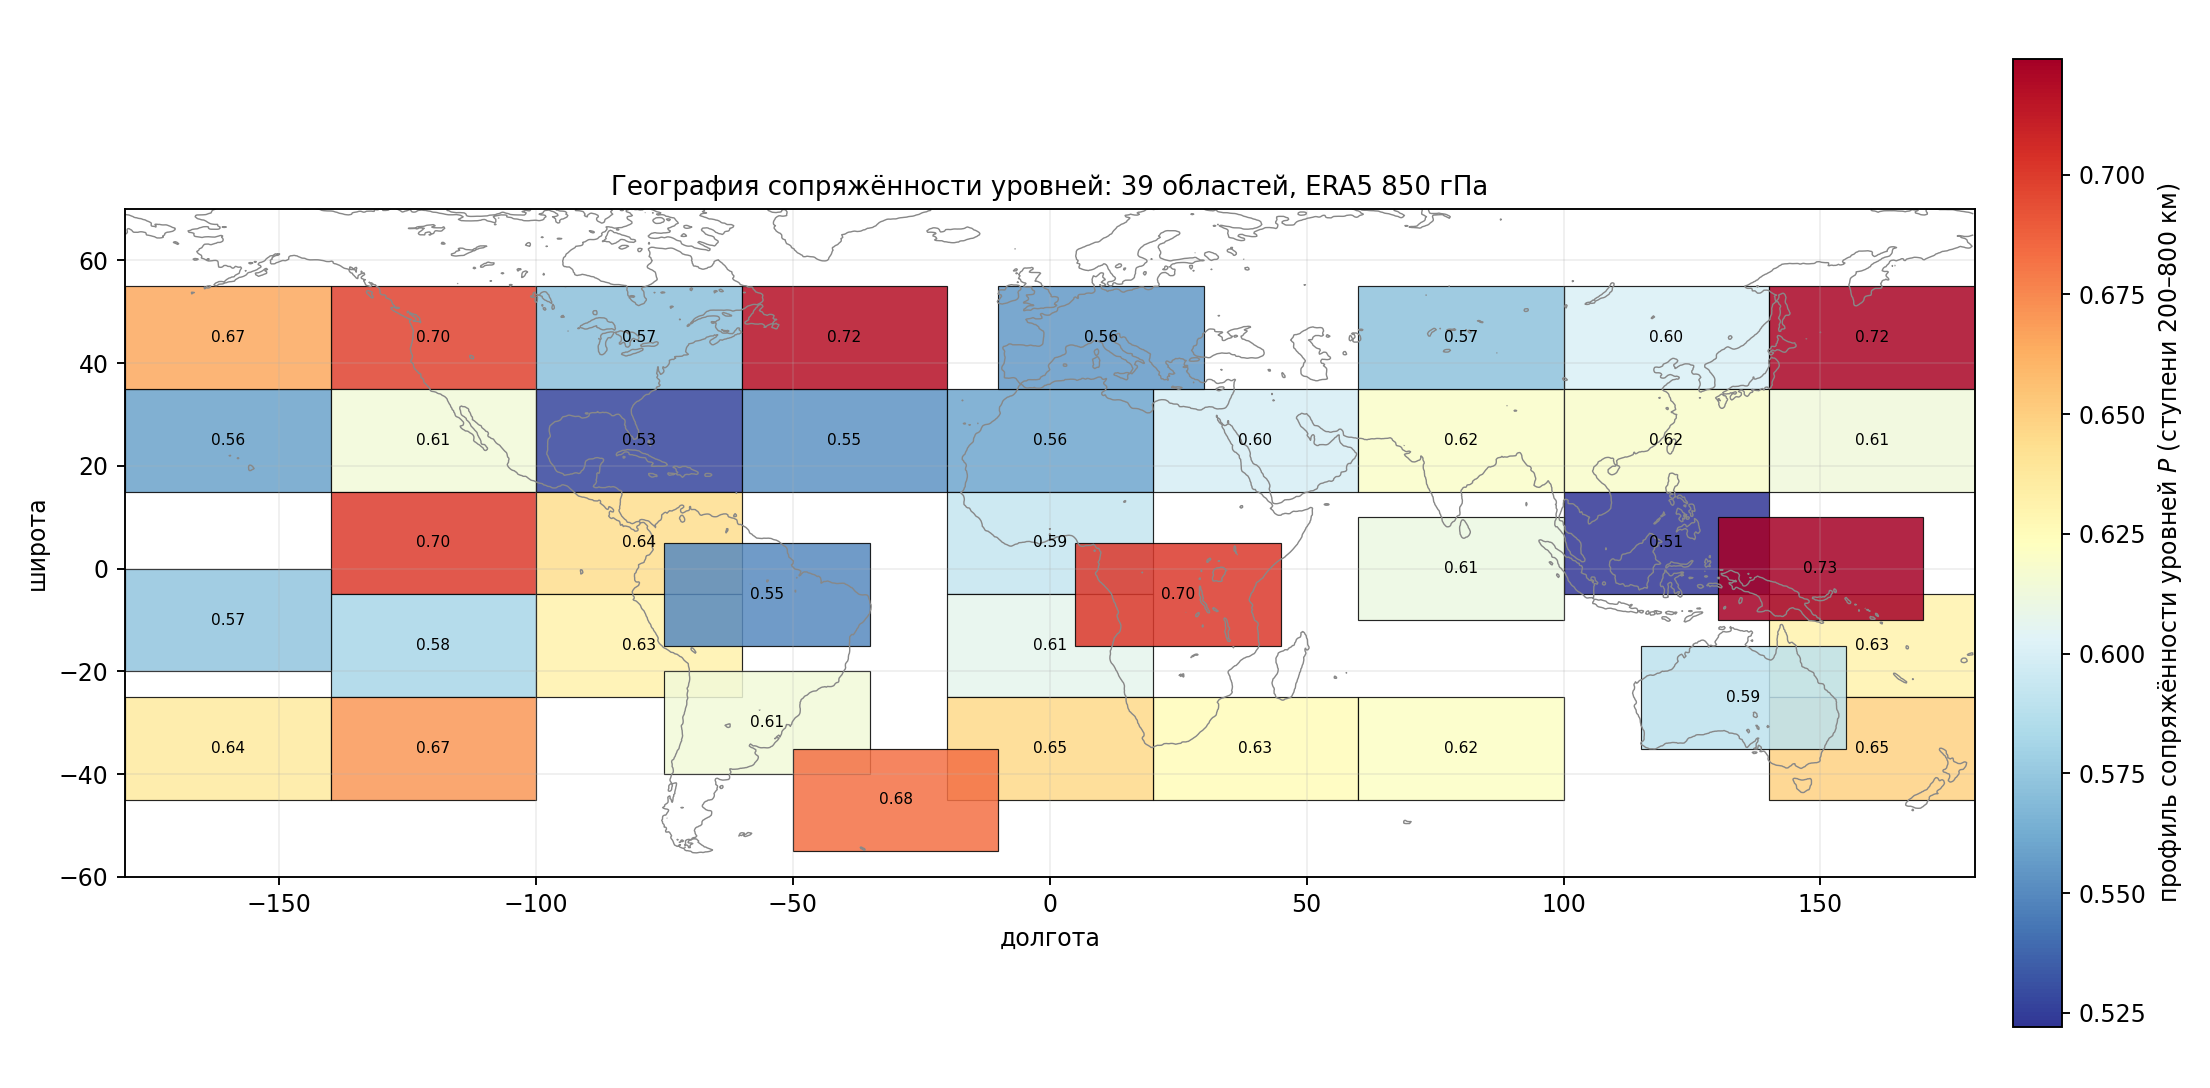
\includegraphics[width=\linewidth]{figures/figP_world_map.png}
\caption{География сопряжённости уровней: средние значения профиля по разрешённым ступеням 4--5 (пары полос 200--400/400--800 и 400--800/800--1600~км) для 39 областей, ERA5, 850~гПа. Двенадцать областей выбраны содержательно, 27 --- формальным решёточным правилом.}
\label{fig:pmap}
\end{figure}

\subsection{Проверка инвариантности: сезоны, годы, ЭНСО, независимый реанализ}
\label{sec:invariance}

Первая группа проверок утверждения~\eqref{eq:invariance} --- устойчивость к смене сезона, года, фазы ЭНСО и источника данных (табл.~\ref{tab:tests}, строки 1--4). Региональная сигнатура подтверждается на 32 отложенных регион-окнах 2021--2022~гг., не участвовавших в построении дескриптора, с большим размером эффекта ($\Delta=+1{,}12$, $p=0{,}001$): межрегиональные расстояния между профилями превышают внутрирегиональные более чем на одну единицу стандартизованного пространства дескрипторов. Сигнатура не сводится к полуфрактальным характеристикам уровней ($\Delta=+0{,}65$ на остатках, $p=0{,}001$), к скаттеринг-статистикам ($\Delta=+0{,}30$, $p=0{,}026$) и к полному спектру мощности ($\Delta=+0{,}34$, $p=0{,}029$); две последние проверки находятся на границе значимости и трактуются с оговоркой разд.~\ref{sec:inference}, а вопрос о спектре окончательно решается контролем равновеликими областями (разд.~\ref{sec:artifacts}). Сигнатура воспроизводится в квазинезависимом реанализе MERRA-2 --- другая модель и система усвоения при общей наблюдательной базе --- как по кластеризации ($\Delta=+1{,}15$, $p=0{,}001$), так и по региональной географии (ранговая корреляция с ERA5 $\rho=0{,}93$ по 12 регионам). Подчеркнём, что проверки последнего типа используют в качестве единицы целый регион, а не регион-окно: согласие географий двух реанализов по 12 областям ($p=1{,}2\cdot10^{-5}$), корреляция $0{,}93$ между двумя независимыми периодами самого ERA5 по 39 областям (разд.~\ref{sec:artifacts}) и согласие $0{,}93$ двух схем разбиения территории --- регион-уровневые проверки межгодовой устойчивости, не зависящие от вопроса об эффективном числе окон.

\begin{table}[H]
\centering
\caption{Сводка проверок профиля сопряжённости. $\Delta$ --- размер эффекта теста кластеризации (разность медианных межрегиональных и внутрирегиональных расстояний в единицах стандартизованного пространства дескрипторов); $p$ --- перестановочный уровень значимости (999 переназначений региональных меток регион-окнам; минимум 0,001). Строки 1--4 --- 32 отложенных регион-окна 2021--2022~гг. и 48 основных 2023--2024~гг.; строки 5--6 --- контроль равновеликими областями.}
\label{tab:tests}
\small
\begin{tabular}{@{}p{0.50\linewidth}p{0.44\linewidth}@{}}
\toprule
Проверка & Итог\\
\midrule
1. Региональная сигнатура: отложенные окна, независимые годы и фазы ЭНСО & $\Delta=+1{,}12$; $p=0{,}001$\\
2. Сверх полуфрактальных характеристик уровней \cite{Krenke2019}; сверх скаттеринг-статистик \cite{Cheng2024} & $\Delta=+0{,}65$; $p=0{,}001$ / $\Delta=+0{,}30$; $p=0{,}026$\\
3. Сверх полного спектра мощности & $\Delta=+0{,}34$; $p=0{,}029$; регрессионный контроль геометрии: $\Delta=+0{,}22$; $p=0{,}10$\\
4. Сигнатура в MERRA-2; согласие географии ERA5--MERRA-2 & $\Delta=+1{,}15$; $p=0{,}001$; $\rho=0{,}93$\\
5. Контроль равновеликими областями: сигнатура; отложенные окна & $\Delta=+1{,}26$; $p=0{,}001$ / $\Delta=+1{,}56$; $p=0{,}001$\\
6. Контроль равновеликими областями: сверх спектра & профиль с поправкой $\Delta=+0{,}22$; $p=0{,}033$; исходный $\Delta=+0{,}35$; $p=0{,}007$\\
7. Только разрешённые ступени 4--5 & $\Delta=+0{,}61$; $p=0{,}002$\\
8. География в расчёте без усвоения наблюдений (39 областей) & $\rho=0{,}71$; $p=0{,}001$; предел метода $0{,}93$\\
\bottomrule
\end{tabular}
\end{table}

\subsection{Исключение артефактов: разрешение, геометрия, наблюдательная система}
\label{sec:artifacts}

Вторая группа проверок исключает три семейства артефактных объяснений.

\emph{Эффективное разрешение.} Мелкие ступени лестницы лежат ниже эффективного разрешения реанализа и могли бы отражать свойства численной диссипации. Контроль, ограниченный разрешёнными ступенями 4--5, сохраняет сигнатуру ($\Delta=+0{,}61$, $p=0{,}002$; табл.~\ref{tab:tests}, строка~7); сопоставления с внешними источниками ведутся только по разрешённым ступеням.

\emph{Геометрия выборки.} Градусные области имеют широтно-зависимые километровые размеры, и часть межрегиональных различий могла быть картографическим отпечатком. Регрессионный контроль --- добавление модуля широты, шага сетки и ширины области в набор контрольных признаков --- сводил сверхспектральную кластеризацию к незначимой ($\Delta=+0{,}22$, $p=0{,}10$; строка~3), оставляя вопрос открытым. Контроль равновеликими областями решает его на уровне построения выборки (рис.~\ref{fig:b18}): при нарезке, устраняющей широтную зависимость геометрии из самой выборки, региональная сигнатура сохраняется на основных и отложенных окнах ($\Delta=+1{,}26$ и $+1{,}56$, оба $p=0{,}001$), география профилей при смене нарезки воспроизводится (объединённая ранговая корреляция <<градусы--километры>> $0{,}93$), а сверхспектральная кластеризация значима: $\Delta=+0{,}22$, $p=0{,}033$ для профиля с суррогатной поправкой и $\Delta=+0{,}35$, $p=0{,}007$ для исходного (строки 5--6). Расхождение двух контролей объяснимо: регрессионные ковариаты поглощали не только геометрию, но и связанный с широтой физический межрегиональный сигнал; контроль построением выборки свободен от этого смешения. Методическая оговорка сохраняется: спектральные признаки сами по себе кластеризуют регионы сильнее профиля ($\Delta=+2{,}54$ на равновеликих областях); утверждение работы всегда состояло не в <<сильнейшей кластеризации>>, а в наличии воспроизводимой информации \emph{сверх} спектра. Два дополнения снимают смежные вопросы о произвольности конструкции. Во-первых, замена фиксированной октавной лестницы на лестницу, масштабированную локальным радиусом деформации, сохраняет региональную сигнатуру профиля с суррогатной поправкой ($\Delta=+1{,}60$, $p=0{,}001$): кластеризация не привязана к конкретному километражу ступеней. Во-вторых, вариация зональной протяжённости равновеликих областей $\pm10\,\%$ меняет отношение сторон области при почти неизменной площади, и профили каждого региона при этом воспроизводятся с $\rho\ge0{,}93$ --- форма области не является скрытым источником сигнала.

\begin{figure}[H]
\centering
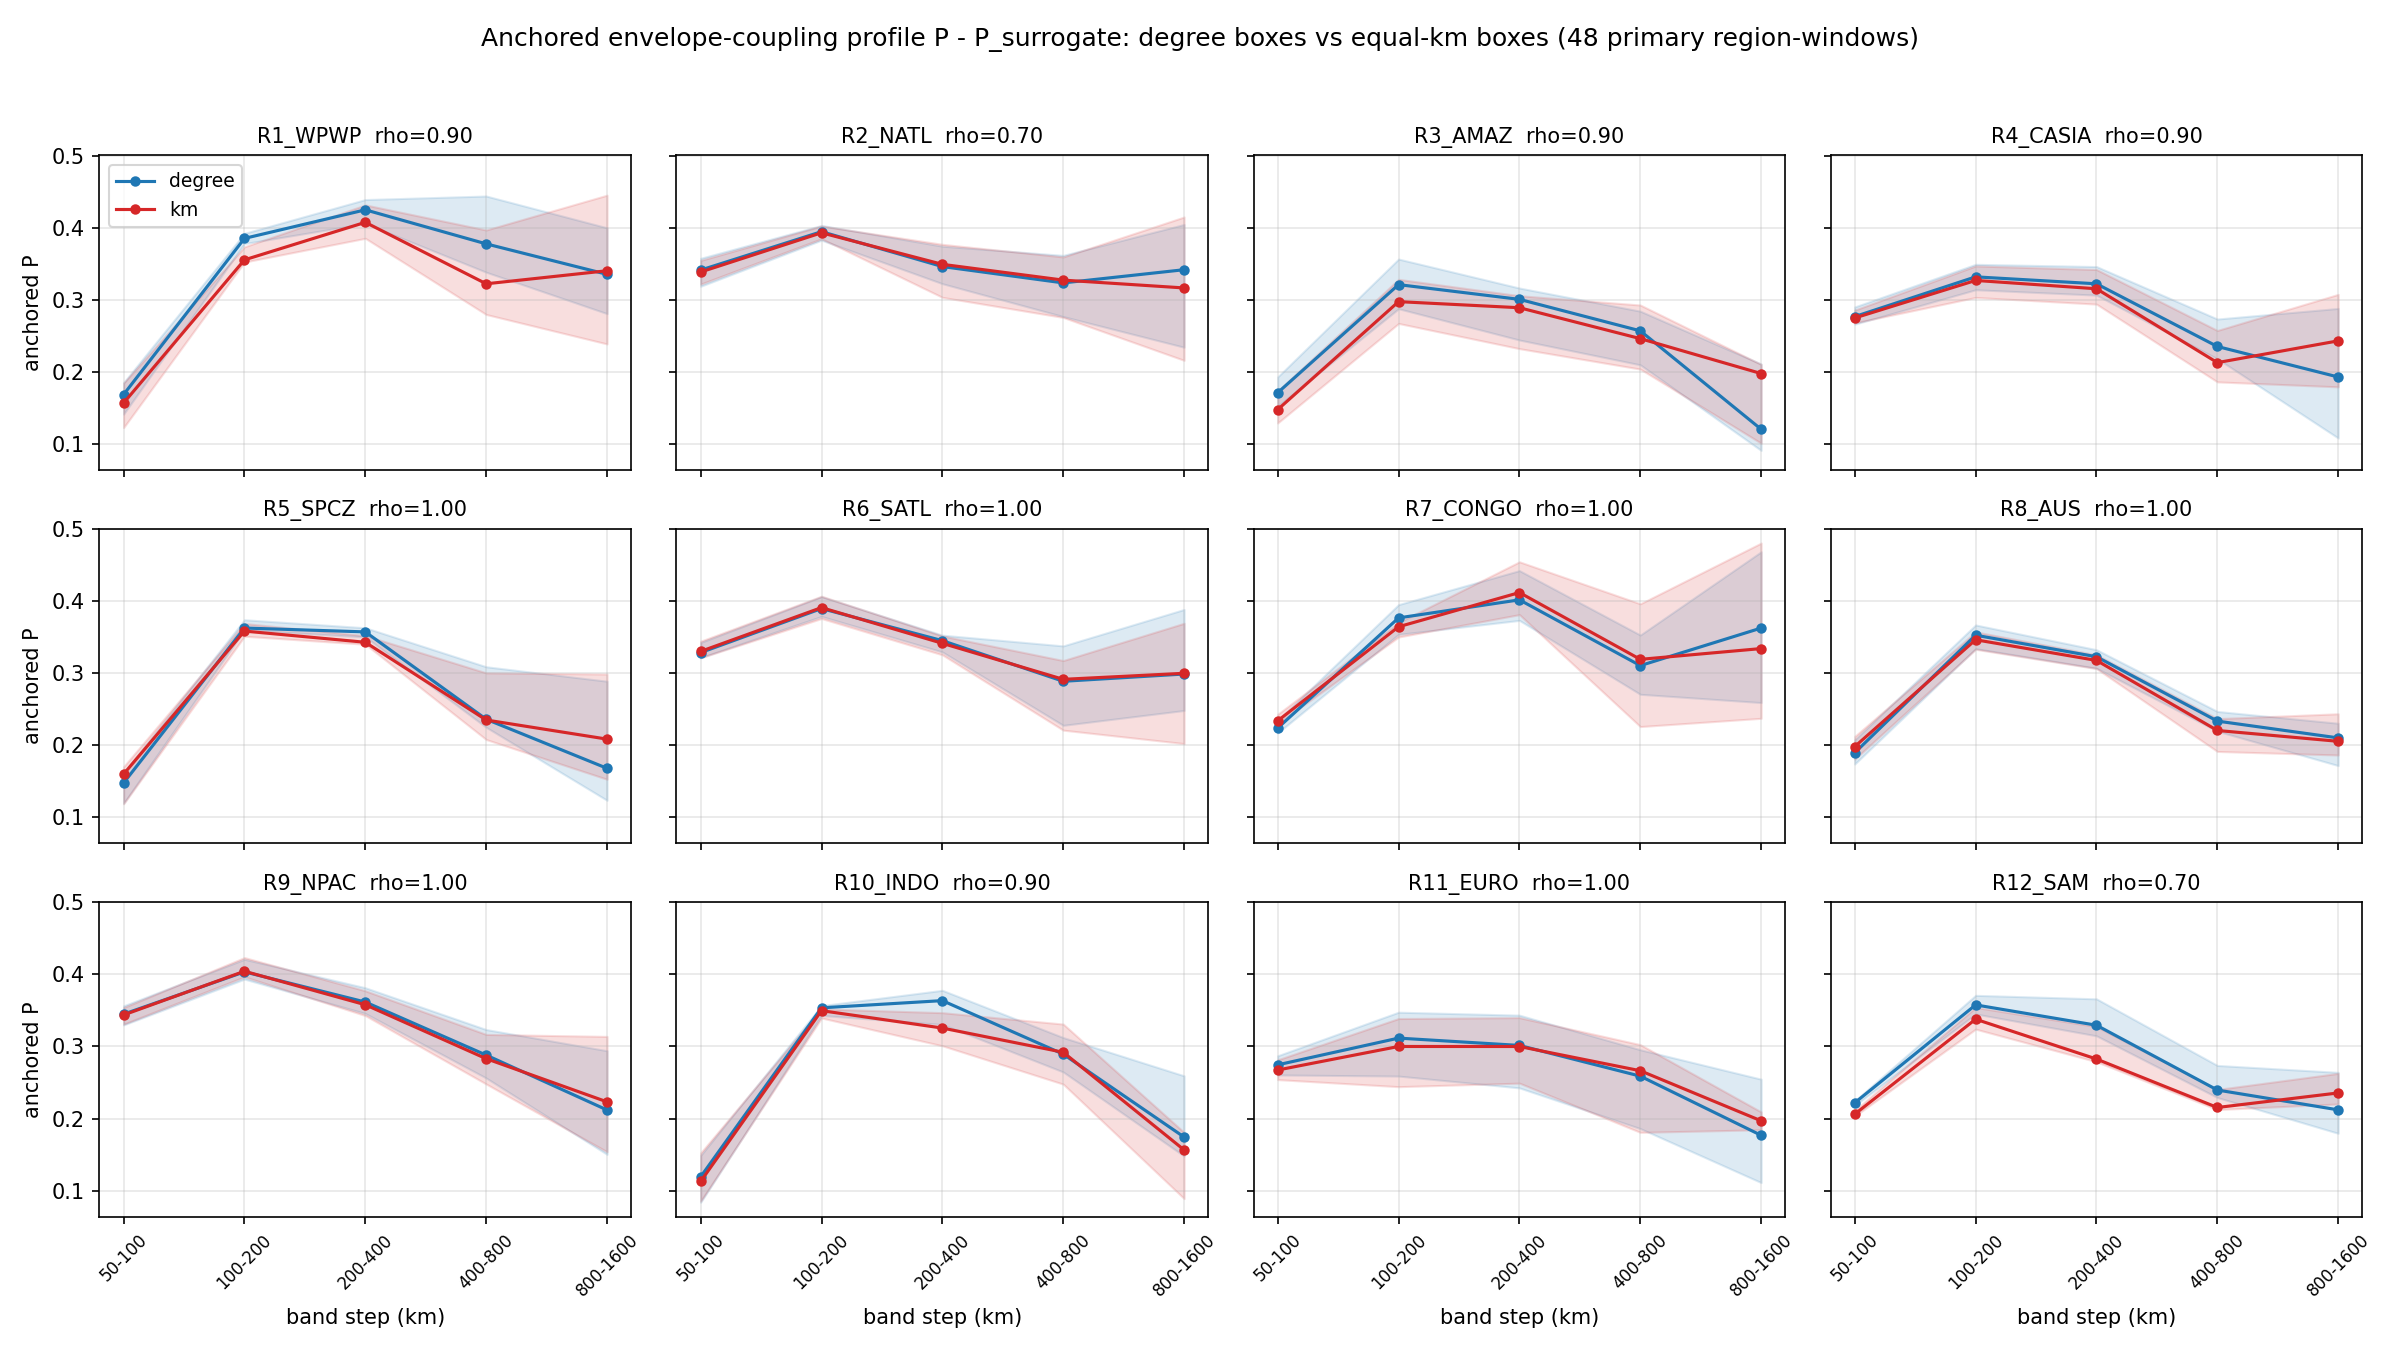
\includegraphics[width=\linewidth]{figures/figP_B18_design_control.png}
\caption{Контроль геометрии построением выборки: профили сопряжённости с суррогатной поправкой $P-P_{\mathrm{surr}}$ на градусных областях $20^\circ\times40^\circ$ (синий) и на равновеликих областях $2000\times2800$~км (красный) для двенадцати регионов, 48 основных регион-окон 2023--2024~гг. Полосы --- размах по окнам; в заголовках --- ранговая корреляция профилей двух нарезок по регионам.}
\label{fig:b18}
\end{figure}

\emph{Наблюдательная система.} Согласие двух реанализов не отделяет свойство атмосферы от свойства наблюдательной сети: ERA5 и MERRA-2 усваивают в основном одни и те же наблюдения \cite{Hersbach2020,Gelaro2017}. Проверкой служит расчёт по свободной модели, не усваивающей наблюдений вовсе (рис.~\ref{fig:free}): региональная география сопряжённости в эксперименте \texttt{highresSST-present} воспроизводит географию ERA5 с ранговой корреляцией $\rho=0{,}71$ ($p=0{,}001$, 39 областей). Оценивать эту величину следует относительно внутреннего предела метода --- корреляция между двумя независимыми периодами самого ERA5 составляет $0{,}93$, --- то есть достигнуто около трёх четвертей возможного; различие естественно, поскольку свободный расчёт воспроизводит климатологию режимов, а не конкретную их реализацию (окна модели относятся к 2014~г., окна ERA5 --- к 2017--2024~гг.; разд.~\ref{sec:data}). Обе величины относятся к \emph{региональному} уровню сопоставления по 39 областям; сопоставление глобальных мозаичных карт дескриптора --- предмет отдельной работы и характеризуется собственными числами.

Корректная формулировка вывода такова: \emph{наблюдаемая региональная структура воспроизводится в свободной модельной интеграции и потому не может быть объяснена только структурой сети атмосферных наблюдений или процедурой их усвоения}. Более сильное утверждение --- о полной независимости от всякого общего для реанализа и модели фактора --- один свободный расчёт дать не может: модель разделяет с реанализом заданную наблюдаемую температуру поверхности океана, родственные параметризации и близкий масштаб эффективного разрешения. Эти ограничения обсуждаются в разд.~\ref{sec:limitations}.

\begin{figure}[H]
\centering
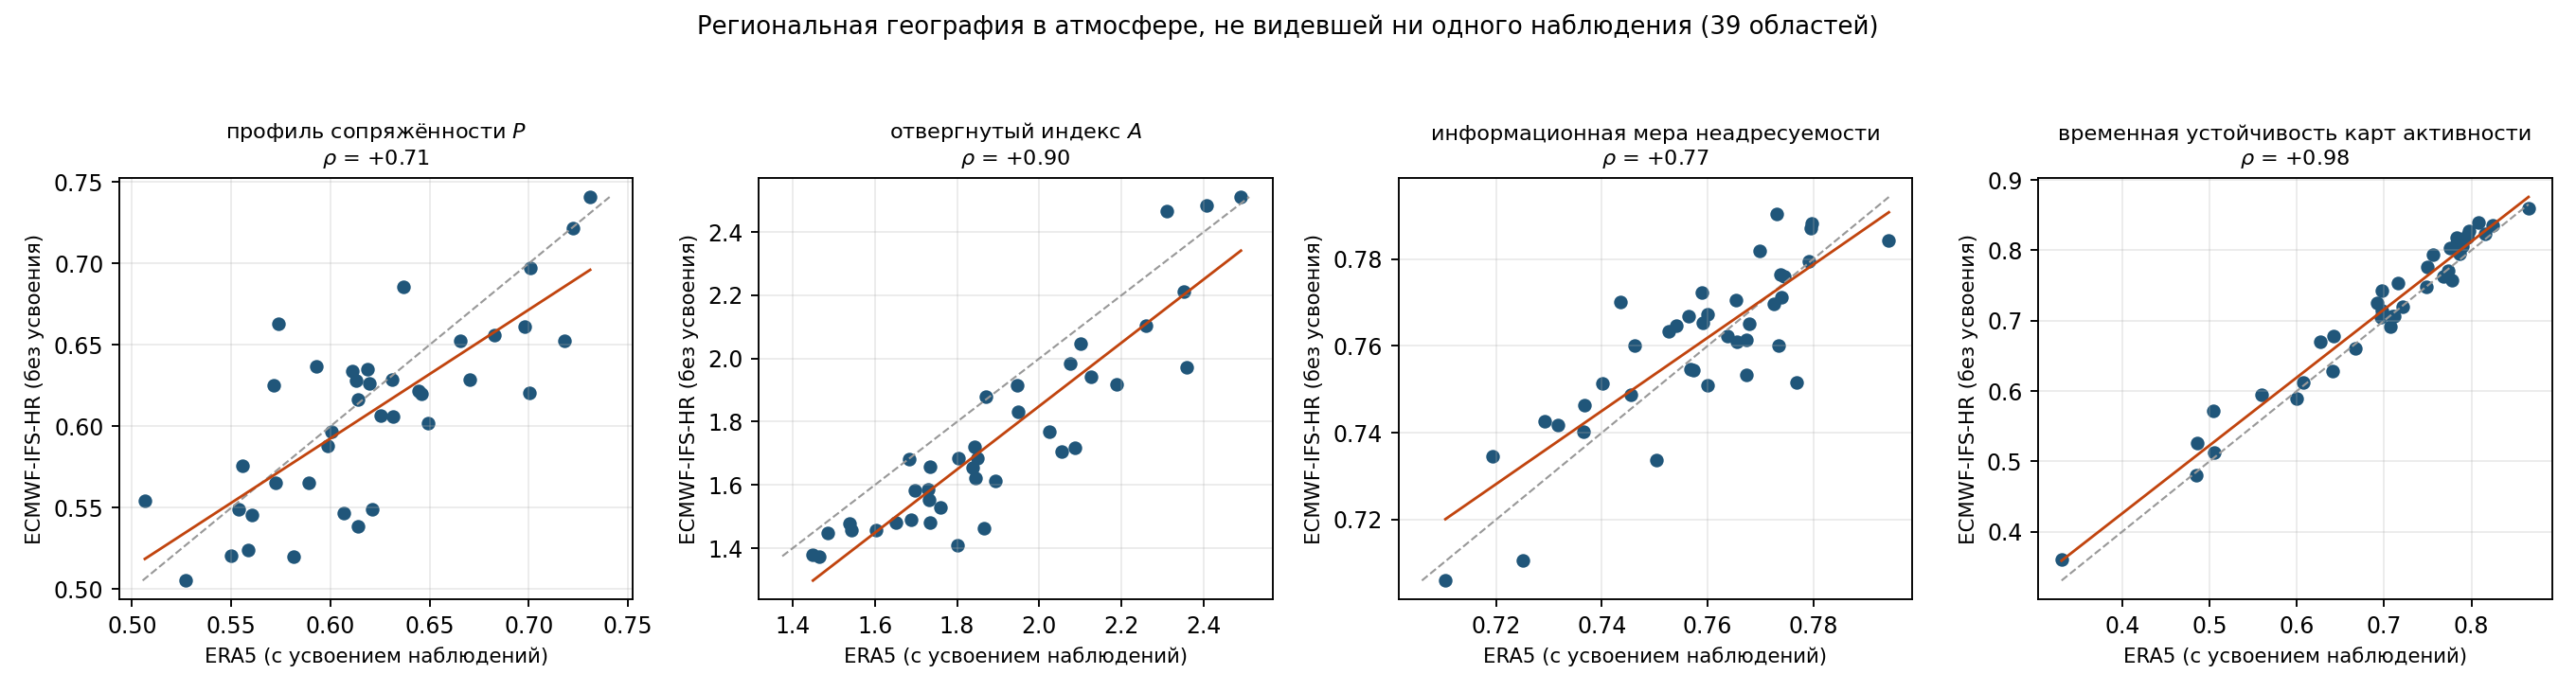
\includegraphics[width=\linewidth]{figures/figP_free_running.png}
\caption{Сопоставление региональной географии по ERA5 (ось абсцисс) и по свободному расчёту ECMWF-IFS-HR без усвоения наблюдений (ось ординат) для 39 областей. Слева направо: профиль сопряжённости $P$; отвергнутый индекс невзаимности $A$; независимая информационная мера межуровневой связи; временная устойчивость карт активности. Пунктир --- линия равенства.}
\label{fig:free}
\end{figure}

\subsection{Что измеряет и чего не измеряет дескриптор}
\label{sec:meaning}

\emph{Проверка содержания.} Независимая мера --- невосстановимость размещения $u_i$. Для каждого срока ранги полей $\ln E_{i-1}$ и $\ln E_i$ по узлам внутренней маски разбиваются на $k=16$ равночастотных корзин; по двумерной гистограмме корзин вычисляется взаимная информация $I_i$, нормируемая на энтропию корзинного распределения ($H=\ln k$ при равночастотном разбиении), и
\begin{equation}
u_i(t)=1-\frac{I_i(t)}{H},
\label{eq:nmi}
\end{equation}
далее, как и для профиля, берётся медиана по срокам окна и среднее по разрешённым ступеням. Ранговое разбиение делает меру инвариантной к монотонным преобразованиям амплитуды, а обращение $1-I/H$ придаёт ей смысл невосстановимости: чем выше $u$, тем слабее размещение мелкого уровня предопределено соседним крупным, поэтому её связь с профилем отрицательна: $\rho=-0{,}93$; при этом связь профиля с амплитудой полосы составляет лишь $+0{,}20$, а с временн\'{о}й устойчивостью карт активности (средней по узлам и разрешённым полосам автокорреляцией огибающей на лаге 6~ч) --- $+0{,}02$. Это не внешняя проверка (обе величины --- статистики одного совместного распределения), но она устанавливает главное: профиль является добросовестной сводкой именно того, насколько размещение мезомасштабной изменчивости предопределено соседним крупным уровнем и не является тенью ни амплитуды, ни инерции поля.

\emph{Отвергнутая конструкция второго дескриптора.} Первоначально наряду с профилем предлагался индекс невзаимности $A$ --- мера непереставимости статистических операторов агрегирования и детализации, которой приписывался смысл необратимости географического обобщения. Индекс воспроизводим (MERRA-2 $\rho=0{,}93$; свободный расчёт $\rho=0{,}90$), однако проверка содержания его не подтвердила: на синтетических полях с управляемой восстановимостью мелкого уровня по крупному индекс на неё не реагирует ($\rho=-0{,}32$ и $-0{,}35$ в двух прочтениях, тогда как независимая информационная мера отзывается корректно в обоих: $0{,}92$--$0{,}93$ по модулю, со знаком, отвечающим ориентации меры в каждом прочтении) и монотонно следует за временн\'{о}й устойчивостью поля ($\rho=1{,}00$ на синтетике; $+0{,}53$ на реальных данных против $+0{,}03$ у информационной меры). Заключение определённое: $A$ --- воспроизводимая характеристика временн\'{о}й устойчивости поля, а не необратимости обобщения; конструкция выведена из основного изложения. Причина ошибки методическая: операторы оцениваются по скользящему окну, и чем медленнее меняется поле, тем систематичнее смещается результат.

\emph{Прочие проверенные и отвергнутые истолкования} сведены в табл.~\ref{tab:negative}; они очерчивают область корректного использования величины. Отдельного упоминания заслуживают два пункта. Дескрипторы не измеряют межмасштабный поток кинетической энергии: прямое сопоставление с потоком, вычисленным методом пространственного огрубления \cite{Germano1992,Aluie2018}, объясняет доли процента его изменчивости. Вертикальной универсальности не обнаружено: на уровне 500~гПа региональная сигнатура статистически не подтверждается при вдвое меньшей выборке, поэтому корректная формулировка --- отсутствие подтверждения, а не доказанное различие.

\begin{table}[H]
\centering
\caption{Проверенные и отвергнутые интерпретации и применения. Первые шесть строк --- проверки содержания величины; последние три --- прикладные гипотезы (разд.~\ref{sec:geo}).}
\label{tab:negative}
\small
\begin{tabular}{@{}p{0.56\linewidth}p{0.38\linewidth}@{}}
\toprule
Проверяемое положение & Итог проверки\\
\midrule
Индекс невзаимности $A$ измеряет необратимость обобщения & отвергнуто (следует за временн\'{о}й устойчивостью поля)\\
Дескрипторы отслеживают межмасштабный поток кинетической энергии \cite{Germano1992,Aluie2018} & отвергнуто (характеристики поля деформации информативнее на два порядка)\\
Форма профилей подчиняется универсальному закону от средовых ковариат & отвергнуто (коллапса к единой кривой нет)\\
Дескрипторы вертикально универсальны (перенос на 500~гПа) & не подтверждено (уровнеспецифичность)\\
Дескрипторы информативны для замыкания влагобюджета реанализа \cite{Trenberth1991,Mayer2021} & отвергнуто\\
Режимная связь с осадками формализуема как уравнение <<источник--сток>> \cite{Masunaga2012,PetersNeelin2006} & не установлено (характерное время $\sim$2~сут частично воспроизводится инерцией процедуры оценивания)\\
Дескрипторы предсказывают скорость роста ошибки ансамблевого прогноза & не подтверждено на имеющихся данных (ошибка управляется бароклинностью: $\rho=+0{,}86$ с модулем широты)\\
Дескрипторы предсказывают уровень мезомасштабной ошибки анализа & не подтверждено на имеющихся данных (связь исчезает после контроля амплитуды)\\
Дескрипторы предсказывают потерю мезомасштаба в моделях машинного обучения \cite{Lam2023,Bi2023,Price2025,Rasp2024} & не подтверждено на имеющихся данных (спектральная характеристика --- более сильный предиктор)\\
\bottomrule
\end{tabular}
\end{table}

\subsection{Географическая интерпретация и границы применимости}
\label{sec:geo}

\emph{Штормовые пути и конвекция.} География дескриптора систематична: максимум сопряжённости --- внетропические штормовые пути, минимум --- влажно-конвективные режимы (разд.~\ref{sec:map}). Содержательная интерпретация этого разделения --- предмет отдельной публикации; здесь фиксируется только сам воспроизводимый рисунок.

\emph{Конго и Амазония.} Показательный случай --- два очага глубокой конвекции над сушей в близких широтах. Существенно для статуса примера: бассейны Конго и Амазонии --- \emph{единственные два} региона глубокой конвекции над сушей в заранее заданном наборе двенадцати областей, так что пара не является результатом перебора вариантов; выбор для иллюстрации сделан после вычислений, но среди заранее заданных кандидатов выбора не было. При сходном режиме увлажнения бассейны обнаруживают качественно различную архитектуру иерархии (рис.~\ref{fig:congo}); различие сосредоточено на верхней ступени профиля: медиана по восьми сезонным окнам каждой области (Конго --- 2021--2024~гг., Амазония --- 2017--2019 и 2023--2024~гг.) составляет $\rho_5=0{,}70$ против $0{,}42$, причём размахи по окнам --- $0{,}57$--$0{,}81$ и $0{,}36$--$0{,}54$ соответственно --- \emph{не перекрываются}. На четвёртой ступени различие медиан составляет лишь $0{,}08$, тогда как на пятой --- $0{,}28$: контраст сосредоточен на верхней разрешённой ступени; значения ступеней ниже эффективного разрешения в аргументации не используются. Контраст устойчив к геометрии выборки: для профиля с суррогатной поправкой (четыре окна 2023--2024~гг.) контраст пятой ступени при переходе от градусных к равновеликим областям сужается с $0{,}242$ до $0{,}136$, сохраняя знак и 56\,\% величины (Амазония $0{,}120\to0{,}198$; Конго $0{,}363\to0{,}334$). Для контекста: у тропических океанических областей набора $\rho_5$ занимает промежуточные значения (0,47--0,69), так что контраст Конго--Амазония --- не край распределения, а различие двух сопоставимых по режиму территорий. Оговорка интерпретации: пара не свободна от неконтролируемых различий --- сезонность осадков, орографическое окружение и антропогенные изменения растительного покрова двух бассейнов различаются, --- поэтому пример демонстрирует различительную способность дескриптора, а не механизм различия.

Содержательно это означает следующее. В бассейне Конго очаги мезомасштабной активности размещаются преимущественно там же, где активен соседний крупный уровень: по крупномасштабному полю можно указать, где окажется мезомасштаб. В Амазонии та же пара уровней распределена почти безразлично: мезомасштабная организация в значительной мере отвязана от крупного поля. Дескриптор различает территории, близкие по стандартным характеристикам режима --- климатологии осадков, конвективной доступной потенциальной энергии и наклону спектра вихря, --- по признаку, прямо относящемуся к задаче генерализации; в этом состоит его непосредственная польза для районирования.

\begin{figure}[H]
\centering
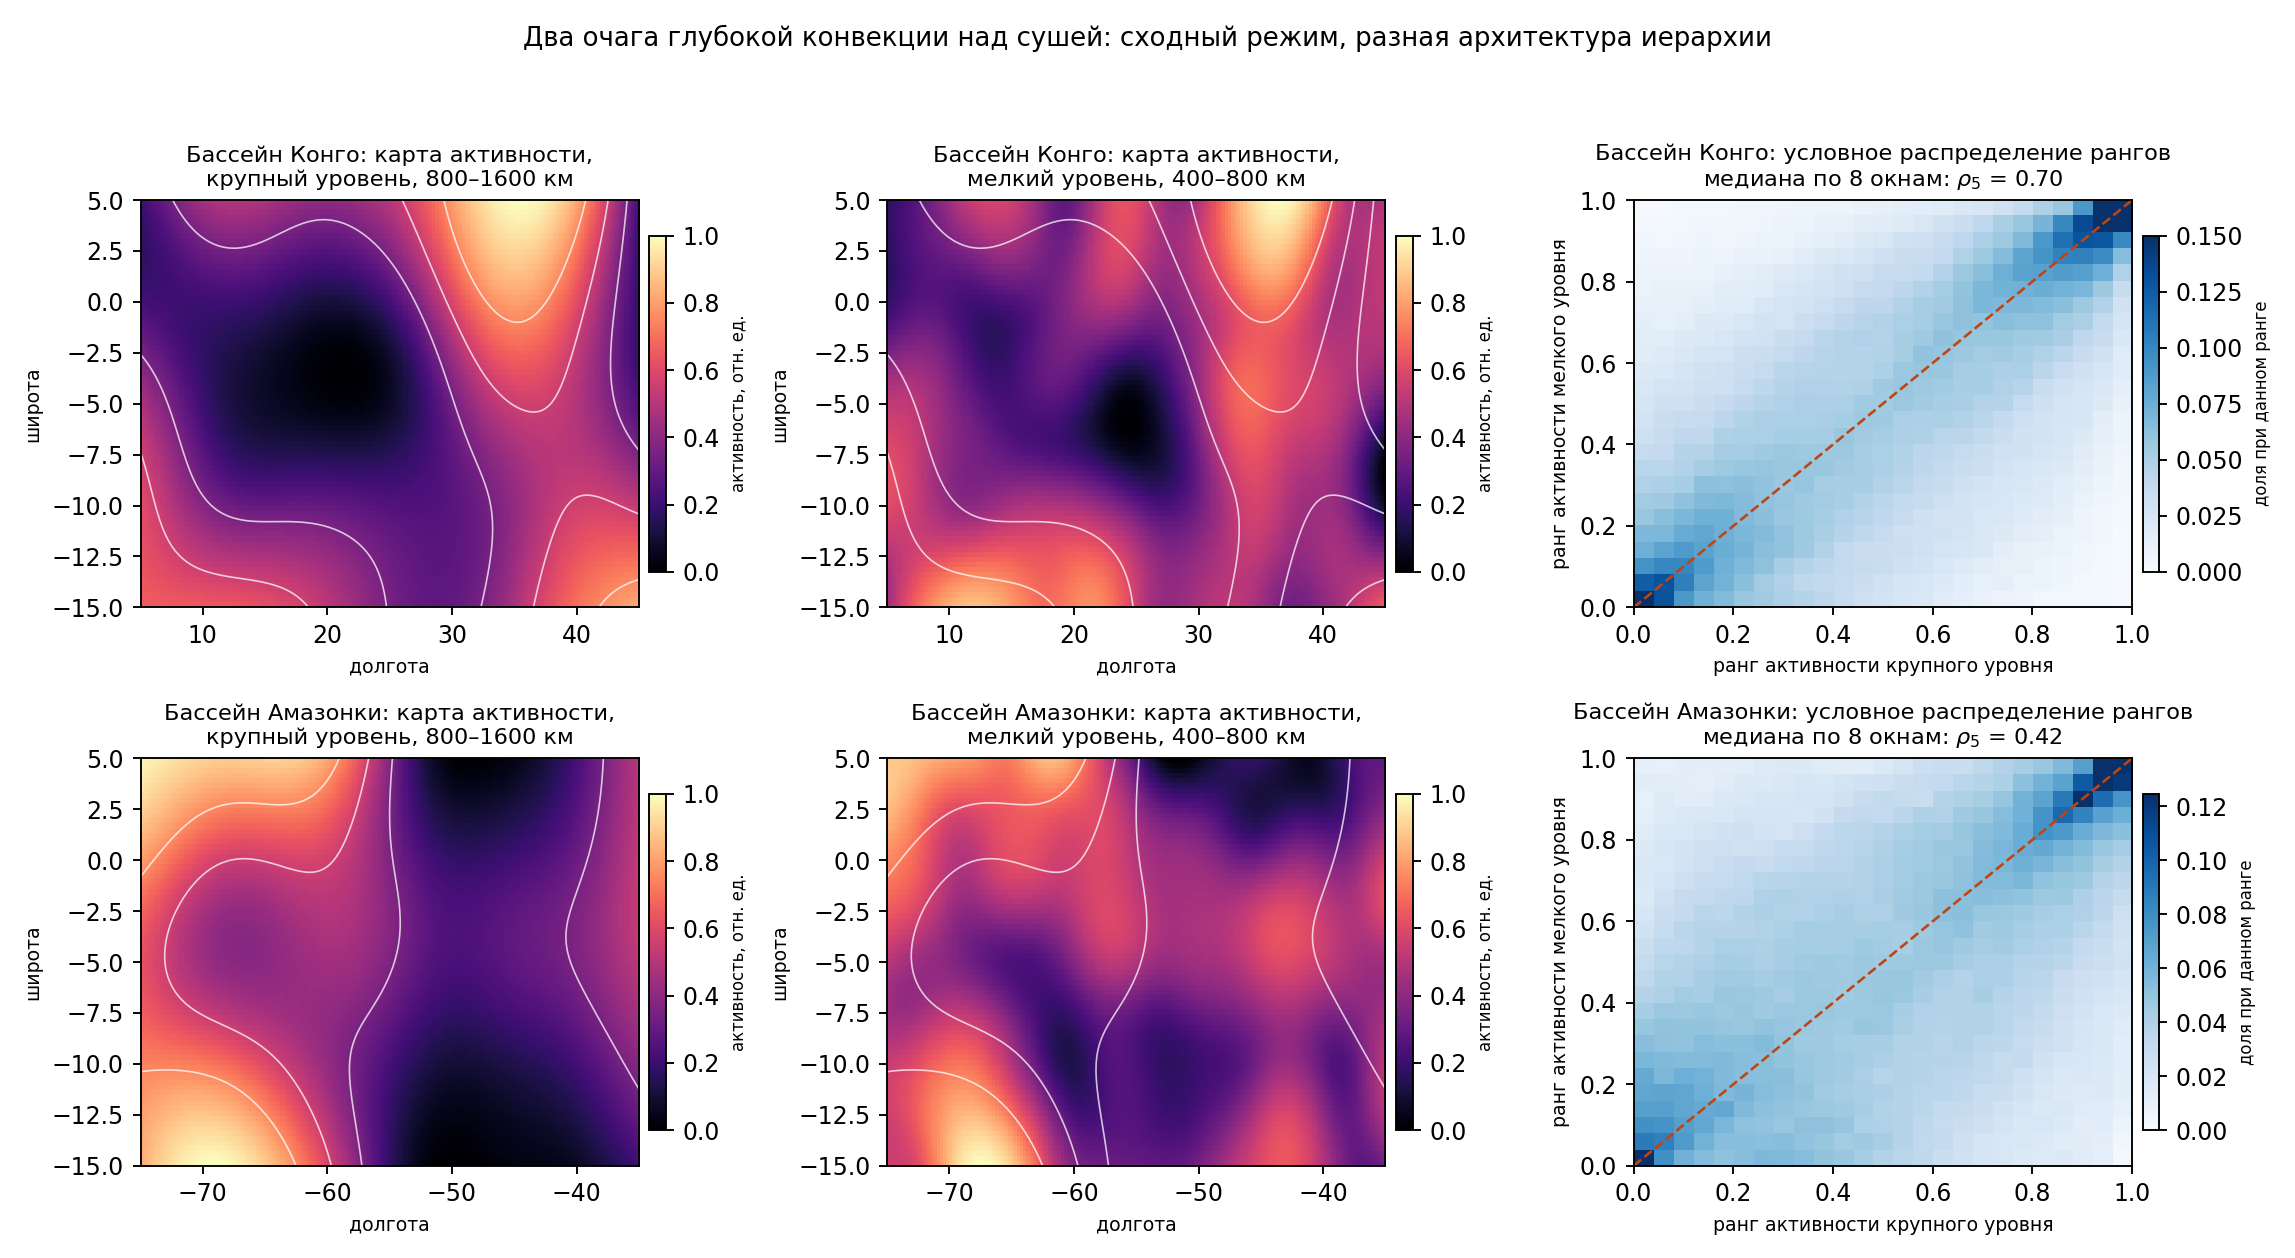
\includegraphics[width=\linewidth]{figures/figP_congo_amazon.png}
\caption{Бассейны Конго (вверху) и Амазонки (внизу), январь--март 2023~г. Слева и в центре --- карты активности крупного (800--1600~км) и мелкого (400--800~км) уровней на один срок; белые изолинии --- активность крупного уровня, одни и те же на обеих картах ряда. Справа --- совместное распределение пространственных рангов активности двух уровней по всем срокам окна; пунктир --- диагональ полного соответствия. В Конго мезомасштабная активность привязана к крупному полю, в Амазонии --- нет.}
\label{fig:congo}
\end{figure}

\emph{Прикладные гипотезы.} Естественное ожидание --- что мера подчинённости мезомасштаба крупному полю говорит о качестве прогноза и об обоснованности статистической детализации --- проверено на трёх независимых постановках (табл.~\ref{tab:negative}, последние строки), и ни одна не подтвердилась: скорость роста ошибки ансамблевого прогноза управляется бароклинностью, мезомасштабная ошибка анализа --- амплитудой поля, а география потери мезомасштаба в нейросетевых моделях погоды предсказывается простой спектральной характеристикой лучше, чем дескриптором. Попутно установлен самостоятельный факт (наш расчёт на платформе сопоставления WeatherBench~2 \cite{Rasp2024} по моделям \cite{Lam2023,Bi2023,Price2025}; протокол в репозитории): на заблаговременности пять суток в полосе 200--800~км мезомасштабную дисперсию теряют те и только те системы, которые вычисляют условное среднее (детерминированные модели --- 55--69\,\%, среднее по генеративному ансамблю --- 85\,\%, физическая модель и отдельная реализация ансамбля --- практически ничего). Отрицательный итог следует читать буквально: на данных, собранных неоднородной наблюдательной сетью, и на моделях, целевые функции которых уничтожают мезомасштабную структуру, отсутствие связи не позволяет заключить ни о наличии, ни об отсутствии прикладного содержания величины; для продвижения нужны наблюдения, однородные по плотности, и модели, сохраняющие мезомасштабную изменчивость.

\section{Обсуждение}
\label{sec:limitations}

По совокупности проверок профиль сопряжённости удовлетворяет утверждению~\eqref{eq:invariance} на всём заявленном классе преобразований $\mathcal{T}$, и в этом операциональном смысле --- в смысле программы инвариантов динамики геосистем \cite{Puzachenko2010} --- является региональным инвариантом. Работа при этом \emph{не} утверждает, что найден универсальный инвариант атмосферной динамики, самостоятельная динамическая переменная или мера межмасштабного переноса: первое ограничено границами разд.~\ref{sec:definition}, второе и третье прямо отвергнуты проверками (табл.~\ref{tab:negative}).

Четыре ограничения заслуживают явной фиксации. Во-первых, проверка независимости от наблюдательной системы опирается на один свободный расчёт одной модели: он исключает объяснение через сеть наблюдений и усвоение, но разделяет с реанализом заданную температуру поверхности океана, родственные параметризации и близкое эффективное разрешение (сопоставление ведётся на общей сетке $0{,}5^\circ$ и только по разрешённым ступеням; при пессимистичной спектральной оценке разрешения ступень 4 частично попадает в серую зону, ступень 5 надёжна при обеих оценках); желательное усиление --- ансамбль свободных реализаций и модель с иным динамическим ядром (расчёт CMCC-CM2-VHR4 доступен в том же архиве HighResMIP; его период тот же, до 2014~г.). Во-вторых, действуют статистические ограничения перестановочной схемы, перечисленные в разд.~\ref{sec:inference}: результаты на границе значимости трактуются осторожно; ключевые имеют $p=0{,}001$, большие размеры эффекта и подтверждение на регион-уровневых проверках. В-третьих, утверждение об инвариантности ограничено полем, уровнем, масштабами и периодом, перечисленными в разд.~\ref{sec:definition}; за их пределами (500~гПа, другие переменные, прогностические применения) свойства величины либо не подтверждены, либо отвергнуты. В-четвёртых, чувствительность к семейству фильтров и ширине сглаживания огибающей не варьировалась (параметры зафиксированы до начала вычислений); её систематическая проверка --- предмет отдельной методической работы.

\section{Выводы}
\label{sec:conclusion}

1.~Предложен дескриптор межуровневой организации атмосферной циркуляции --- профиль сопряжённости октавных уровней $P$ --- с полным операциональным описанием: поле, лестница масштабов, операторы уровня и огибающей, маска, форма корреляции, агрегирование и суррогатная поправка зафиксированы протоколом до вычислений (табл.~\ref{tab:params}). Ранговая форма корреляции --- техническая деталь реализации, а не источник новизны ($\rho=0{,}99$ с линейной формой); родственные формы оценки известны в других дисциплинах, и новизна работы состоит в свойствах измеряемого объекта, а не в статистике.

2.~Профиль удовлетворяет заранее сформулированному утверждению условной инвариантности~\eqref{eq:invariance}: региональная сигнатура сохраняется при смене сезона, независимого года, фазы ЭНСО ($\Delta=+1{,}12$, $p=0{,}001$ на отложенных выборках), источника данных (MERRA-2: $\Delta=+1{,}15$, $p=0{,}001$; география $\rho=0{,}93$) и схемы разбиения территории, и не сводится к спектру мощности: при контроле равновеликими областями сверхспектральная кластеризация значима ($\Delta=+0{,}22$, $p=0{,}033$ для профиля с суррогатной поправкой; $\Delta=+0{,}35$, $p=0{,}007$ для исходного), тогда как регрессионный контроль геометрии оставлял вопрос открытым. За пределами этого класса преобразований свойства величины не проверялись либо отвергнуты (разд.~\ref{sec:limitations}).

3.~Региональная география дескриптора воспроизводится в свободном модельном расчёте, не усваивающем атмосферных наблюдений ($\rho=0{,}71$ при внутреннем пределе метода $0{,}93$; региональный уровень сопоставления, 39 областей): наблюдаемая структура не может быть объяснена только устройством наблюдательной сети или процедурой усвоения. Полное отделение от факторов, общих для модели и реанализа (заданная температура океана, параметризации), требует ансамбля свободных расчётов и остаётся задачей дальнейшей работы.

4.~Наибольшая сопряжённость свойственна внетропическим штормовым путям, наименьшая --- влажно-конвективным режимам. Бассейны Конго и Амазонии --- единственные два очага глубокой конвекции над сушей в заранее заданном наборе регионов --- различаются архитектурой иерархии с неперекрывающимися размахами по окнам ($\rho_5$: 0,57--0,81 против 0,36--0,54), и контраст сохраняется при контроле равновеликими областями. Дескриптор различает территории, близкие по стандартным характеристикам режима, и в этом качестве продолжает линию инвариантов организации геосистем --- от выделения уровней к измерению их взаимодействия.

5.~Границы применимости установлены прямыми проверками: дескриптор не измеряет межмасштабный поток кинетической энергии; вертикальная универсальность не подтверждена; три прикладные гипотезы --- о скорости роста ошибки прогноза, об уровне мезомасштабной ошибки анализа и о потере мезомасштаба в нейросетевых моделях --- не подтверждены на имеющихся данных, причём в каждом случае более сильным предиктором оказалась простая характеристика фонового состояния: бароклинность (модуль широты), амплитуда поля и спектральный наклон соответственно. Отрицательный результат воспроизводим и очерчивает требования к данным, при которых вопрос о прикладном содержании может быть поставлен заново.

6.~Первоначально предлагавшийся второй дескриптор --- индекс невзаимности операторов агрегирования и детализации --- сохраняет статус воспроизводимой региональной характеристики, но приписанное ему истолкование как меры необратимости обобщения отвергнуто прямой проверкой содержания: величина следует за временн\'{о}й устойчивостью поля, а не за восстановимостью мезомасштаба.

\paragraph{Доступность данных и кода.} Исходные данные --- открыто доступные продукты сторонних поставщиков и в репозитории автора не дублируются: поля ERA5 доступны через Climate Data Store (Copernicus Climate Change Service), данные MERRA-2 --- через NASA GES DISC, модельные расчёты HighResMIP --- через Earth System Grid Federation; доступ к первым двум требует бесплатной учётной записи. Код анализа, скрипты получения исходных данных, полные протоколы проверок с заранее фиксированными критериями, журнал отступлений и производные табличные результаты, достаточные для воспроизведения всех рисунков и статистических проверок работы, открыты в репозитории \url{https://github.com/Theclimateguy/Shroedinger} (версия v6.1; постоянный архив версий --- Zenodo, DOI 10.5281/zenodo.19565769). Маршрут воспроизведения статьи --- от получения данных до каждой строки табл.~\ref{tab:tests} --- описан в файле \texttt{reproducibility/article1\_README.md} и автоматизирован скриптом \texttt{reproducibility/reproduce\_article1.py}; там же приведены контрольные суммы ожидаемых артефактов и проверочный маршрут на одном регион-окне, не требующий массовой загрузки данных.

\printbibliography[title={Список литературы}]

\end{document}
